\documentclass[journal=esthag,manuscript=article]{achemso}
%%%%%%%%%%%%%%%%%%%%%%%%%%%%%%%%%%%%%%%%%%%%%%%%%%%%%%%%%%%%%%%%%%%%%
%% Place any additional packages needed here.  Only include packages
%% which are essential, to avoid problems later. Do NOT use any
%% packages which require e-TeX (for example etoolbox): the e-TeX
%% extensions are not currently available on the ACS conversion
%% servers.
%%%%%%%%%%%%%%%%%%%%%%%%%%%%%%%%%%%%%%%%%%%%%%%%%%%%%%%%%%%%%%%%%%%%%
\usepackage[T1]{fontenc}       % Use modern font encodings
\usepackage[utf8]{inputenc}
\usepackage{todonotes}
\usepackage{amsmath}

%%%%%%%%%%%%%%%%%%%%%%%%%%%%%%%%%%%%%%%%%%%%%%%%%%%%%%%%%%%%%%%%%%%%%
%% If issues arise when submitting your manuscript, you may want to
%% un-comment the next line.  This provides information on the
%% version of every file you have used.
%%%%%%%%%%%%%%%%%%%%%%%%%%%%%%%%%%%%%%%%%%%%%%%%%%%%%%%%%%%%%%%%%%%%%
%%\listfiles

%%%%%%%%%%%%%%%%%%%%%%%%%%%%%%%%%%%%%%%%%%%%%%%%%%%%%%%%%%%%%%%%%%%%%
%% Place any additional macros here.  Please use \newcommand* where
%% possible, and avoid layout-changing macros (which are not used
%% when typesetting).
%%%%%%%%%%%%%%%%%%%%%%%%%%%%%%%%%%%%%%%%%%%%%%%%%%%%%%%%%%%%%%%%%%%%%
\newcommand*\mycommand[1]{\texttt{\emph{#1}}}


%%%%%%%%%%%%%%%%%%%%%%%%%%%%%%%%%%%%%%%%%%%%%%%%%%%%%%%%%%%%%%%%%%%%%
\author{Eduard Szöcs}
\affiliation[Institute for Environmental Sciences]{Institute for Environmental Sciences, University of Koblenz-Landau, Germany}
\email{szoecs@uni-landau.de}
\phone{+49 (0)6341 280 31552}

\author{Marvin Brinke}
\affiliation[German Federal Institute of Hydrology]{German Federal Institute of Hydrology (BfG), Koblenz, Germany}

\author{Bilgin Karaoglan}
\affiliation[German Federal Environmental Agency]{Federal Environmental Agency (UBA), Dessau-Roßlau, Germany}

\author{Ralf B. Schäfer}
\affiliation[University Koblenz-Landau]{Institute for Environmental Sciences, University of Koblenz-Landau, Germany}


%%%%%%%%%%%%%%%%%%%%%%%%%%%%%%%%%%%%%%%%%%%%%%%%%%%%%%%%%%%%%%%%%%%%%
\title[Pesticides small streams]{Pesticides pollution of small streams in Germany}
\abbreviations{mo, pest, ger, tu}
\keywords{Monitoring, Pesticides, Germany, Toxic Units, Freshwater}


%%%%%%%%%%%%%%%%%%%%%%%%%%%%%%%%%%%%%%%%%%%%%%%%%%%%%%%%%%%%%%%%%%%%%
\begin{document}
%%%%%%%%%%%%%%%%%%%%%%%%%%%%%%%%%%%%%%%%%%%%%%%%%%%%%%%%%%%%%%%%%%%%%
%% The "tocentry" environment can be used to create an entry for the
%% graphical table of contents. It is given here as some journals
%% require that it is printed as part of the abstract page. It will
%% be automatically moved as appropriate.
%%%%%%%%%%%%%%%%%%%%%%%%%%%%%%%%%%%%%%%%%%%%%%%%%%%%%%%%%%%%%%%%%%%%%
\begin{tocentry}

Some journals require a graphical entry for the Table of Contents.
This should be laid out ``print ready'' so that the sizing of the
text is correct.

Inside the \texttt{tocentry} environment, the font used is Helvetica
8\,pt, as required by \emph{Journal of the American Chemical
Society}.

The surrounding frame is 9\,cm by 3.5\,cm, which is the maximum
permitted for  \emph{Journal of the American Chemical Society}
graphical table of content entries. The box will not resize if the
content is too big: instead it will overflow the edge of the box.

This box and the associated title will always be printed on a
separate page at the end of the document.

\end{tocentry}



%%%%%%%%%%%%%%%%%%%%%%%%%%%%%%%%%%%%%%%%%%%%%%%%%%%%%%%%%%%%%%%%%%%%%
\begin{abstract}
Fehlt noch...
\end{abstract}


%%%%%%%%%%%%%%%%%%%%%%%%%%%%%%%%%%%%%%%%%%%%%%%%%%%%%%%%%%%%%%%%%%%%%
\section{Introduction}

More than 50\% of the total land area in Germany are used by agriculture \citep{statistisches_bundesamt_bodenflache_2014}.
In the year 2014 more the 45,000 tonnes of 766 authorized pesticides were sold for application on this area \citep{bundesamt_fur_verbraucherschutz_und_lebensmittelsicherheit_absatz_2015}.
The applied pesticides may enter surface waters via spray-drift, edge-off-field run-off or drainage, with run-off being one of the major input routes \citep{schulz_comparison_2001,liess_determination_1999}.
Once entered the surface waters pesticides are frequently detected in environmental monitoring \citep{malaj_organic_2014} and may have adverse effects on biota and ecosystem functioning \citep{schulz_field_2004, schafer_effects_2007}.

National monitoring programs are setup for determination and surveillance of the chemical and ecological status of surface, ground and drinking water.
These monitoring programs produce huge amounts of data, which possibly can also be used to answer other questions.
In Germany monitoring programs are setup by the federal states in compliance with the Water Framework Directive \citep{quevauviller_water_2008} and further state specific needs.
However, currently there is no curated national-wide compilation of this data.

Small water bodies are important refuges of biodiversity \citep{davies_comparison_2008} and enabling downstream colonisation of polluted streams \citep{liess_analyzing_2005}.
At the same time they may be exposed to a high risk of pesticide contamination from adjacent agricultural areas and low dilution effects \citep{liess_determination_1999}.
Although small streams comprise a major fraction of streams \citep{nadeau_hydrological_2007} relatively little is know about their chemical and ecological status.

The aim of this study was to compile monitoring data on a national scale and to answer the questions: \\
(i) Can the currently available monitoring data used for a representative description of the pollution situation? \\
(ii) Are small agricultural waters more polluted compared to bigger streams? Are there thresholds in these relationships? \\
(iii) baHow polluted are small streams and which pesticides are responsible?


\section{Methods}
\subsection{Data compilation}

We queried chemical monitoring data of pesticides from sampling sites with catchment size $\mathrm{< 100km^2}$ for the years 2005 to 2015 from all 13 non-city federal states of Germany.
Additionally, we compiled data available from previous studies and searched online databases.
This yielded to a total of more then 30 datasets of different formats.
In the following we will use the ISO 3166-2:DE standard abbreviations for federal states.

We homogenized and unified these datasets into a common database.
We implemented a robust and transparent data cleaning work flow \citep{poisot_best_2015}, though parts of the dataset are proprietary.
An overview of the data cleaning process is provided in the supplemental materials.  
To assess whether samples were taken during potential rainfall events we intersected sampling coordinates with daily precipitation data \citep{rauthe_central_2013} from the sampling date and the day before.

\subsection{Characterization of chemical pollution}
We characterized chemical pollution (excluding sum parameters) using three indicators:

\begin{enumerate}
  \item National and international Environmental Quality Standards (EQS) \citep{ogewv_verordnung_2011,european_union_directive_2013}:
  We used only Maximum Annual Concentration EQS (MAC-EQS) for characterization.
  These were available for 29 compounds (Supplement, Table xxx\todo{ref}).

  \item Regulatory Acceptable Concentrations (RAC) \citep{brock_linking_2010}:
  This is the lowest concentration at which no acceptable biological effects are expected. 
  These are derived during authorization  process of pesticides and contain an uncertainty factor.
  The German Federal Environmental Agency provided RACs for 105 compounds (Supplement, Table xxx\todo{ref}).  
  We expressed RAC as Risk Quotient (RQ):
  \begin{equation}
  RQ = \frac{C}{RAC}
  \end{equation}
  Where $C$ is the concentration of a compound in a sample.

  \item Maximum Toxic Units ($\mathrm{TU_{max}}$)  \citep{sprague_measurement_1970}: 
  \begin{equation}
  TU_{max} = max(\frac{C_i}{EC_{50, D.magna, i}})
  \end{equation}

  Where $C_i$ is the concentration of compound $i$ in a sample and $EC_{50, D.magna, i}$ is the concentration of this compound where 50\% of the exposed animals showed after 48 hours an effect in a laboratory study.
  We compiled $EC_{50, D.magna}$ values from literature \citep{malaj_organic_2014}, databases \citep{lewis_international_2016,u.s._epa_ecotoxicology_2015} or model predictions \citep{schuurmann_quantitative_2011}, where experimental data had priority.
  We could compile $EC_{50, D.magna}$ values for 384 compounds (Supplement, Table xxx\todo{ref}))
  We used the maximum TU per sample, as it is independent of the number of measured compounds and makes no assumptions on the mode of action.
  A table of all included compounds can be found in the supplement.
\end{enumerate}


\subsection{Characterization of catchments}
We delineated catchments upstream of the sampling sites using a digital elevation model \citep{eea_digital_2013} and a multiple flow direction algorithm \citep{holmgren_multiple_1994} as implemented in GRASS GIS 7 \citep{neteler_grass_2012}.
Catchment delineation has been manually checked for accuracy. 
In areas with low relief energy the delineation algorithm did not produce accurate results and we used river catchments provide by federal state authorities in these cases.
For each catchment we calculated the relative coverage (\%) with agricultural areas based on Official Topographical Cartographic Information System (ATKIS) of the land survey authorities.


\subsection{Statistical analyses}

All data-processing and analyses have been performed using R, version 3.3.1 \citep{r_core_team_r:_2016}.
To display differences in the spectra of analysed compounds between federal states we used Multidimensional Scaling (MDS) based on Jaccard dissimilarity in conjunction with hierarchical clustering using the vegan package \citep{oksanen_vegan:_2016}.
We expected non-linear responses to agriculture and catchment size and therefore, used generalized additive models (GAM) to identify relationships \todo{citation fewster}.

We modeled the number of RAC exceedances (No) as:

\begin{align}
\begin{split}
  No_i \sim NB(\mu_i, k) \\
  E(No_i) = \mu_i~and~Var(No_i) = \mu_i + \frac{\mu_i^2}{k} \\
  log(\mu_i)= \beta_0 + f_1(Agri_i) + f_2(Size_i) + log(n_i)
\end{split}
\end{align}

where $No_i$ is the observed number of exceedances at site $i$, $Agri_i$ the proportion of agriculture within the catchment and $Size_i$ the catchment size of the site. 
We used the number of samplings ($n$) as an offset to account different sampling efforts. 
We modeled $No_i$ as resulting from a negative binomial distribution ($NB$).
$f_1$ and $f_2$ are smoothing functions using thin plate regression splines.
The degree of smoothness was estimated using restricted maximum likelihood \todo{cite and check wood 2011}.
Similar models were fitted to the number of EQS-exceedances and the 95th percentile of $log(TU_{max})$ (see Supplement for details).
GAM were fitted using the mgcv package \todo{citation mgcv}.


\section{Results}
\subsection{Overview and representativeness of compiled data}

The compiled dataset comprised only few standing waters (58 sites) and the majority (90\%) of samples where taken via grab sampling.  % see clean.R for numbers
Therefore, we report only results of grab samples from streams. 
The analysed dataset comprised 42236 samples from 3049 sampling sites.  %see do_overview.R for numbers.
We found big differences in the number of sampling sites between federal states (Figure \ref{fig:fig1} and Supplement, Table \todo{Set ref to table}).


\begin{figure}
  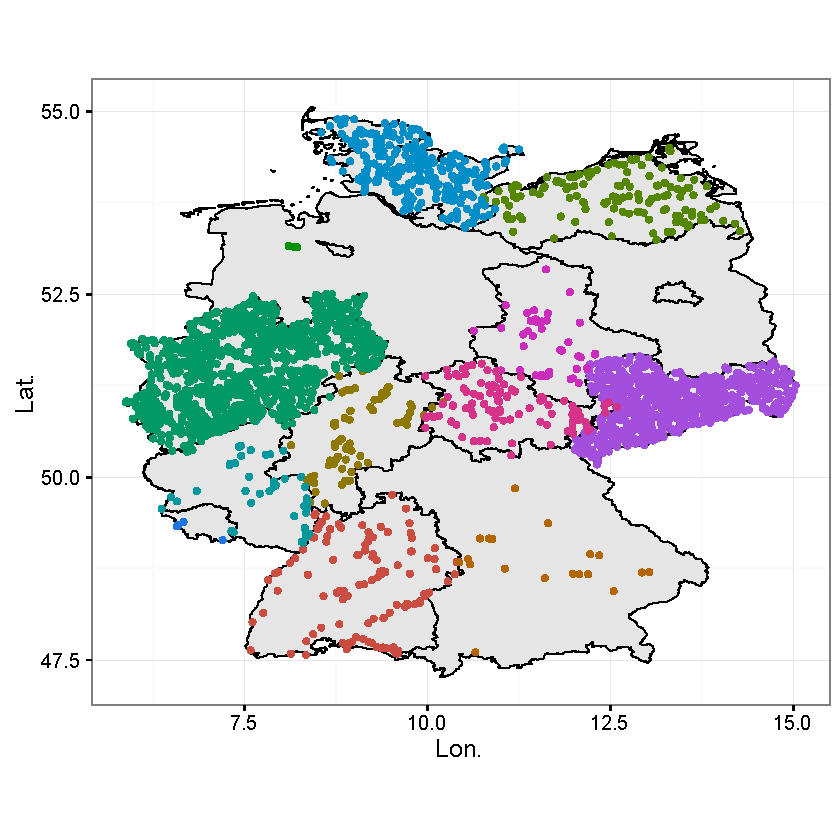
\includegraphics[width=.7\textwidth]{fig/fig1.pdf}
  \caption{Spatial distribution of the 3109 sampling sites. Colour codes different federal states.}
  \label{fig:fig1}
\end{figure}


In total 484 different compounds that could be classified as pesticides and their metobalites were measured at least once (Supplement, Table \todo{Set ref to table}). 
Most of the compounds were herbicides (179), followed by insecticides (117) and fungicides (109).
We found substantial differences of the spectra of analysed compounds (Figure \ref{fig:figvar}).
Hierarchical clustering revealed three groups of states:
i) with less then 100 compounds (SL, ST and TH), ii) with a medium sized spectra and iii) with a big and distinct spectra (RP and NI).
Only 5\% of the samples were taken at or after days with rainfall events greater than 10mm / day.

\begin{figure}
  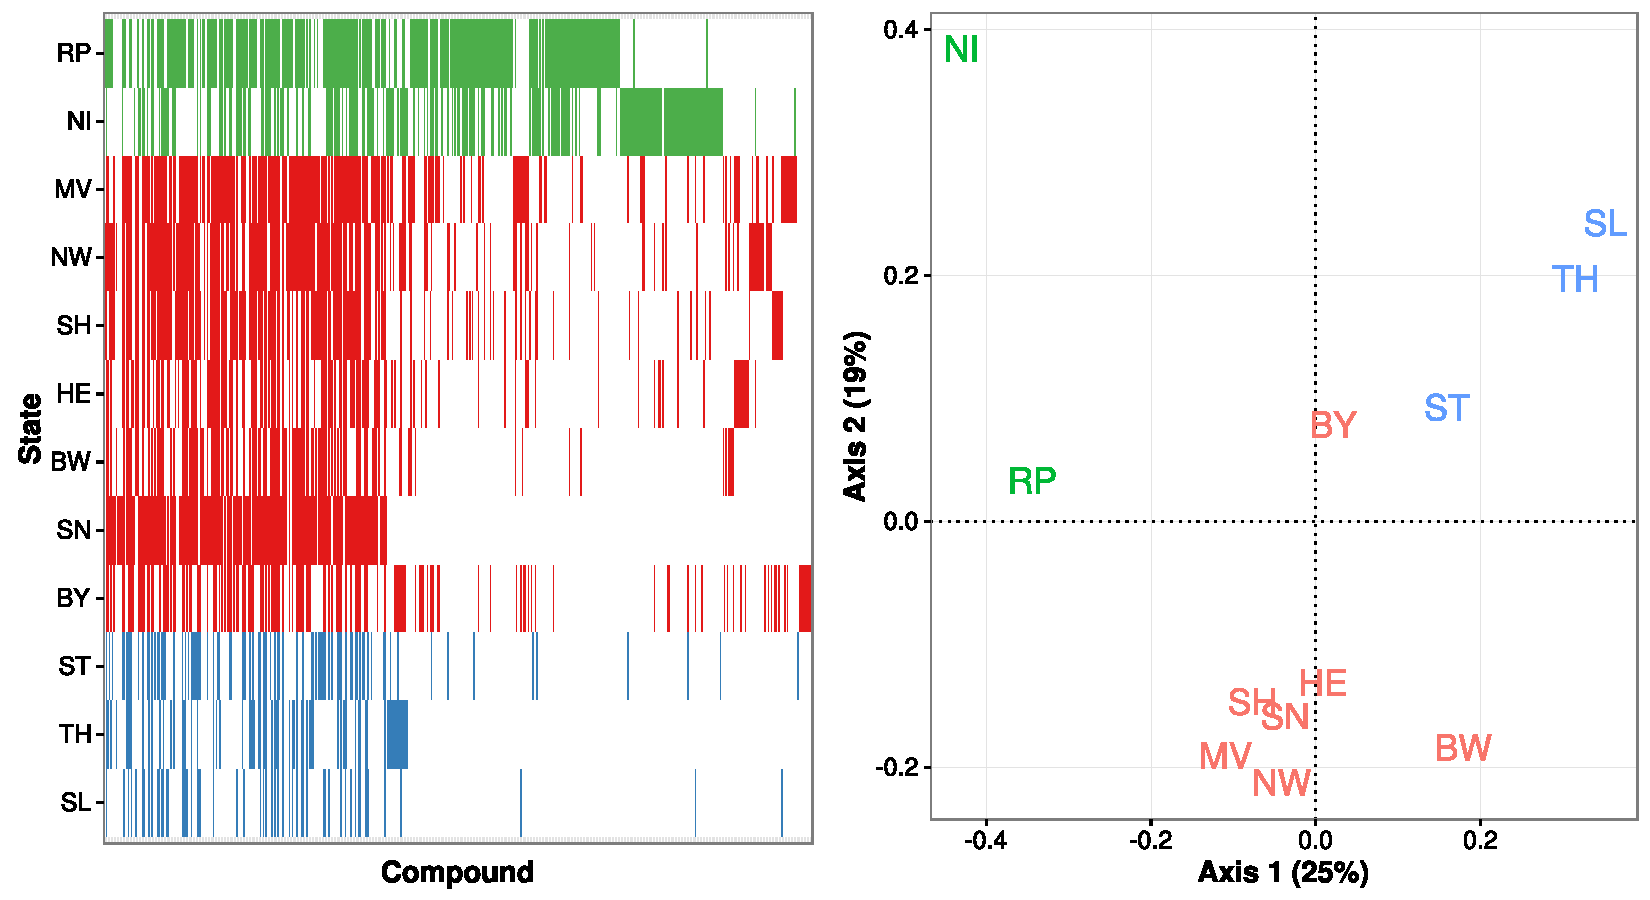
\includegraphics[width=\textwidth]{fig/figvar.pdf}
  \caption{Compound spectra of the different federal states. Left: Barcode plot - Each vertical line is an analysed compound. Right: MDS ordination. 
  Colors according to three groups determined by hierarchical clustering (see Supplement Figure (xxx).}
  \label{fig:figvar}
\end{figure}
\todo{prettify figure!}

We were able to derive for 2376 sites catchment sizes and the proportion of agriculture within catchments. \todo{Check why there are so many missing in BW, NW, RP, SN and TH = phchsitesinfo}.
The distribution of sampling sites across catchment area and agricultural area in the catchment revealed a sharp decline in the distribution of catchment-sizes below $10~km^2$, with most sampling sites with catchments between 10 and 25 $km^2$ (Figure \ref{fig:figezglu}).
The proportion of agriculture in the catchments decreased with increasing catchment size.

\begin{figure}
  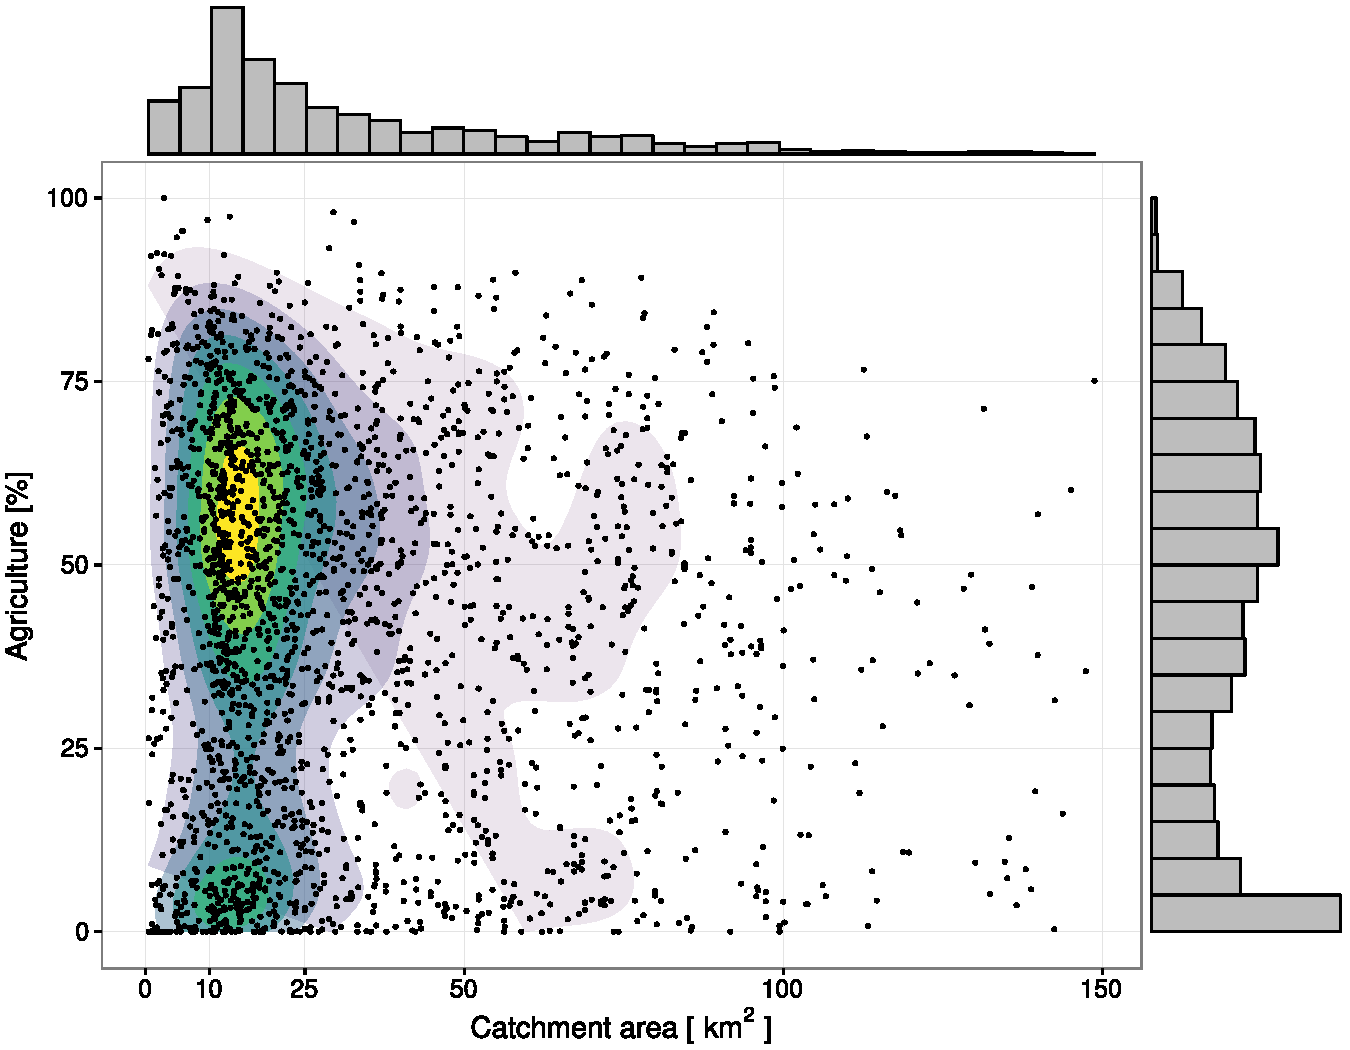
\includegraphics[width=.8\textwidth]{fig/ezglu.pdf}
  \caption{Distribution of catchment area and agriculture within the catchment area across the sampling sites.
  Only sampling sites with catchment area < 150 km\textsuperscript{2} are displayed. 
  Colour codes the 2-dimensional density of points.
  }
  \label{fig:figezglu}
\end{figure}

\todo{1-2 worte das es nicht überall möglich war ezg größe zu bestimmen.}


\subsection{Are small agricultural waters more polluted compared to bigger streams?}

\begin{figure}
  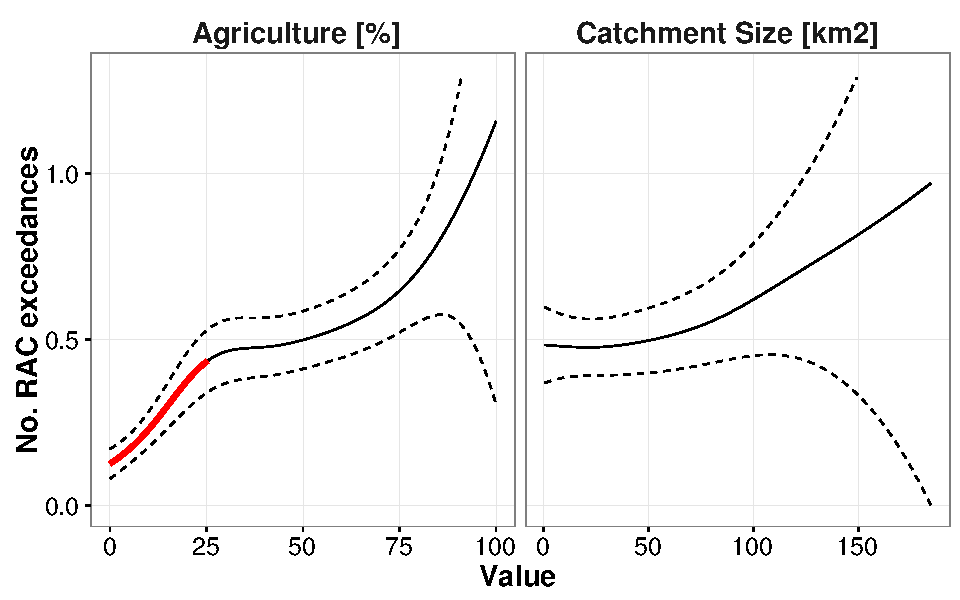
\includegraphics[width=\textwidth]{fig/figrac.pdf}
  \caption{Effect of agriculture within the catchment (left) and catchment size (right) on the number of RAC exceedances. Red line marks statistically significant increases.
  }
  \label{fig:figrac}
\end{figure}



\subsection{Pesticide pollution of small streams}




\section{Discussion}

% Vergleich mit der Schweiz.....

%%% Risk assessment
% findings from field studies on pesti-
% cide exposure and effects must be used for a retrospec-
% tive validation of the current EU regulatory risk assess-
% ment, particularly for its future development.

% validation of the risk assessment through
% targeted chemical and biological post-authorization
% monitoring programs must be implemented for com-
% pounds of concern to ensure that their application


% underestimation of grab sampling (Stehle et al. 2013). 

\subsection{Representativeness of the data}

\subsection{Influence of catchment area and agriculture}

\subsection{Pollution of streams}



%%%%%%%%%%%%%%%%%%%%%%%%%%%%%%%%%%%%%%%%%%%%%%%%%%%%%%%%%%%%%%%%%%%%%
\begin{acknowledgement}
The authors thank the authorities for providing chemical monitoring data and the German Federal Environmental Protection Agency (UBA) for funding this project.
\end{acknowledgement}


%%%%%%%%%%%%%%%%%%%%%%%%%%%%%%%%%%%%%%%%%%%%%%%%%%%%%%%%%%%%%%%%%%%%%
\begin{suppinfo}
The following files are available free of charge.
\begin{itemize}
  \item Supplemental\_Materials.pdf : Supplemental Materials
\end{itemize}
\end{suppinfo}



%%%%%%%%%%%%%%%%%%%%%%%%%%%%%%%%%%%%%%%%%%%%%%%%%%%%%%%%%%%%%%%%%%%%%
\bibliography{references}

\end{document}
